\documentclass[a4paper]{article}
\usepackage{graphicx}
\usepackage{onecolpceurws}
\usepackage{url}
\usepackage{pifont}

\title{Embedded OCL Integration and Debugging}

\author{
Edward D. Willink \\ Willink Transformations Ltd.\\
                Eclipse Modeling Project, \\ \url{http://www.eclipse.org/modeling}
}

\institution{}




\begin{document}
\maketitle

\begin{abstract}
The Object Constraint Language (OCL) is a specification language that is also in principle executable. One of the most useful execution tools is a debugger, and last year Dresden OCL introduced support for debugging as an independent application.  In practice, execution may occur within a variety of host applications and so provision of useful OCL tool support is challenging. In this paper we examine the OCL integration needed for embedded applications and see how the Eclipse OCL debugger supports them.  
%\keywords{OCL, OCL in Ecore, OCL in UML, OCL debugger, OCL integration}
\end{abstract}
\vskip 32pt

\section{Introduction}
A debugger animates the execution of a program so that selected execution states can be inspected in order to shed light on unexpected run-time behaviors. A good debugger provides powerful easy-to-use facilities that enable the programmer to resolve problems rapidly and learn from mistakes.

The Object Constraint Language (OCL)\cite{OCL-2.4} is now over 20 years old, but it was only last year that a true source level OCL debugger became available as part of Dresden OCL\cite{DresdenOCL-Debug}. This is despite consistent observations that a debugger was one of the most important omissions in OCL tool sets\cite{Chimiak-Opaka}.

OCL 1.x was originally specified as part of UML 1.x. OCL 2.0 was separated from UML 2.0 in recognition of the more general utility of OCL, however this leaves OCL by itself incomplete and almost useless. Without models to navigate there is no point in having powerful navigation capabilities. OCL only becomes useful once embedded in a model-providing application.

A variety of tools support development and animation of OCL source text. Very few support use as part of a larger application. This is the focus of this paper. The larger model-providing application may be based on 

\begin{itemize}
\item UML\cite{UML-2.5} (or Ecore\cite{EMF}) models enriched by OCL invariants, operation bodies and property initializers
\item a model transformation language such as QVT\cite{QVT-1.2} or MOFM2T\cite{MOFM2T} with OCL queries
\item proprietary applications that exploit the rigor of compact side-effect-free OCL queries
\end{itemize}

%OCL tool developers cannot easily control the embedding applications and so additional independent OCL-only tools such as an interactive OCL Console provide useful learning and practicing capabilities.

The limitations of OCL do not change when we have a debugger. OCL by itself is almost useless and so an OCL debugger too is almost useless. The user has an OCL related problem in their larger application, the user therefore wants a debugger that works to solve the problem where it occurs. If the user is required to recreate the problem in a standalone OCL debugger, difficult to reproduce problems vanish and so the user is only slightly better off than with the following debugging approaches.

\subsection{OCL Debugging approaches}

In the absence of a useable OCL debugger, OCL programmers are forced to resort to inferior approaches.

Trial and Error: Try, try again until it works.

Divide and Conquer: Try something simpler that works and then elaborate.

Printf: Unfortunately OCL has no `printf' capability and so the traditional approach, of adding debug print out until the problem manifests itself, is not available to OCL programmers\footnote{Eclipse OCL provides oclLog() for this purpose}.

Interactive Console: An interactive console allows an OCL expression to be entered and evaluated and so makes the divide and conquer approach more practical. The user practices the first part of an OCL expression, then extends to include a second part and so forth till the problem is solved. However this requires the user to at least `re-type' the OCL and recreate the problem context in the console tool.

Extended OCL Debugger: OCL debugging is available in some OCL-extending tools such as Eclipse QVTo, and so there is a debugging option that involves wrapping the OCL expression of interest up inside a QVTo transformation and arranging for the OCL expression to be executed in a suitable data context.

Host Debugger: Although no debugger may be available for OCL, a debugger may be available for the OCL tooling. It is therefore possible to debug OCL within the context of the tooling. However this requires understanding of the tool source code and may require many lines of tool code to be stepped for each OCL term.

\subsection{Overview}

None of the above debugging approaches are very satisfactory and so it is hardly surprising that IDE4OCL\cite{Chimiak-Opaka} stresses the need for a debugger.

Dresden OCL\cite{DresdenOCL-Debug} and Eclipse OCL\cite{OCL-Luna} now provide a debugger, but is it usable? For OCL students, it surely is. For more general OCL usage, we need to dig deeper.

In Section  \ref{OCL-Integration} we look at a variety of ways in which OCL may be used with or without the help of framework facilities such as those described in Section \ref{Framework-Integration}. In Section \ref{Launching} we examine different ways in which a debugger may be launched.  Section \ref{Related-Work} examines related work and Section \ref{Conclusion} concludes.

\section{OCL Integration}\label{OCL-Integration}

The OCL specification identifies two different forms of OCL.

Essential OCL comprises just the query capability and so must be embedded within some application to provide modeling context and query activation.

\begin{verbatim}
    kids.kids->isEmpty()
\end{verbatim}

Complete OCL provides an embedding within a textual syntax that enables OCL queries to be used to complement a referenced metamodel with invariants, operation bodies and derived properties. A Complete OCL document solves the problem of a modeling context, but requires an additional application to provoke any execution.

\begin{verbatim}
package example
context Node
inv NoGrandChildren: kids.kids->isEmpty()
endpackage
\end{verbatim}

OCL is of very limited use by itself and so it must be embedded in some application to make OCL usable. In this section we consider various forms of integration within an embedding application that enable OCL to be executed and so add value to the embedding application. These options are summarized in Table \ref{IntegrationOptions} where the first two columns show applicability to Essential OCL or Complete OCL and the subsections in which the approach is discussed further. The remaining columns indicate whether the approach can contribute to an embedding application and whether embedding can use an OCL Toolkit Application Programming Interface (API) or a general modeling Framework.

\begin{table}[ht]
\begin{center}
\caption{Integration Options}\label{IntegrationOptions}
\bigskip
\begin{tabular}{|l|c|c|c|c|c|}
\hline
Integration Approach & Essential OCL & Complete OCL & Embedded & API & Framework\\ \hline \hline
Independent & (\ref{IndependentCompleteOCL}) &\ref{IndependentCompleteOCL} & - & - & -\\ \hline
Integrated & \ref{IntegratedEssentialOCL} & \ref{IntegratedCompleteOCL} & \ding{52} & \ding{52} & \ding{52}\\ \hline
Extended & \ref{ExtendedEssentialOCL} & (\ref{ExtendedEssentialOCL}) & \ding{52} & \ding{52} & \ding{54}\\ \hline
Compiled & \ref{CompiledEssentialOCL} & (\ref{CompiledEssentialOCL}) & \ding{52} & \ding{52} & \ding{52}\\ \hline
\end{tabular}
\end{center}
\end{table}

\subsection{Independent Complete OCL (or  Essential OCL)}\label{IndependentCompleteOCL}

The simplest form of integration is to provide a tool that loads the Complete OCL document, the complemented metamodel and a model comprising conforming instances. 

The user may then request that some or all invariants are executed on some or all instances and receive a report of any violations.

Alternatively, the user may select a metamodel class as context, type a query in an interactive console and request that the result be evaluated. The query may invoke queries defined in the Complete OCL document.

This form of integration can be provided as part of an OCL toolkit independent of other modeling applications.

Essential OCL expression cannot be independent. However, the support for independent Complete OCL may allow an Essential OCL expression to be evaluated interactively.

\subsection{Integrated Essential OCL}\label{IntegratedEssentialOCL}

Essential OCL expressions can be embedded in models such as UML or Ecore to define their behavioral aspects. These may then be used when the embedding application that uses the models also uses an OCL-defined facility.

An OCL toolkit may provide an API to enable an embedding application to exploit OCL. OCL can then be used in embedding applications that choose to use the API. Since there is no standard for the API, the embedding application must explicitly commit to a particular OCL toolkit.

Alternatively an embedding application may use a framework that provides the flexibility for the OCL toolkit to make contributions. OCL is then usable in all embedding applications that use the framework even if they had no intention of supporting OCL.

\subsection{Integrated Complete OCL}\label{IntegratedCompleteOCL}

A Complete OCL document may be used to add value to a embedding application if that application provides support for OCL.

Invariants may contribute to model validation performed by the embedding application.

Queries may define the behavior of operations and properties for the embedding application.

As with Essential OCL integration, an OCL toolkit may provide an extensibility API for explicit use by the embedding application or implicit use as a consequence of underlying framework extensibility.

The way in which the Eclipse Modeling Framework (EMF)  enables Eclipse OCL to contribute additional validations to Xtext is discussed in Section \ref{ResourceSet}.

\subsection{Extended Essential OCL (or Complete OCL)}\label{ExtendedEssentialOCL}

A language, such as QVT that extends OCL, exploits OCL queries as  part of the extended language. Usage of OCL therefore occurs explicitly whenever the extended language needs to evaluate one of these queries.

An extended OCL application is inherently using OCL and so must exploit an API provided by an OCL toolkit. It may also be able to exploit or even extend the code generator provided by an OCL toolkit.

Complete OCL could also form the basis of an extended language, however Complete OCL is something of a dead end. The syntax is not suitable for extension and the behavior requires a further application to complement.

\subsection{Compiled Essential OCL (or Complete OCL)}\label{CompiledEssentialOCL}

Direct embedding of OCL in an application requires the embedding application to incur the parsing costs of the OCL on at least the first use, and potentially the limited execution speed of interpreted execution on every use. If the OCL is compiled to perhaps Java or C++, the parsing costs are incurred during preparation of the embedding application and the execution can be much faster.

An OCL toolkit may provide an OCL to Java code generator with an appropriate API for the embedding application to support OCL explicitly. Alternatively the OCL toolkit may arrange for the generated code to be useful to an extensible framework that a more general embedding application exploits and so supports OCL implicitly.

\section{Framework Integration}\label{Framework-Integration}

As noted above, integration of OCL with an embedding application may be achieved by explicit use of an OCL toolkit API by the embedding application, or by extensibility offered by a framework used by many applications.

Explicit use of an OCL toolkit requires the application to provide the explicit support and to make a choice among competing toolkits.

In contrast, a framework such as EMF may provide a variety of useful modeling services for an application and so, support for OCL may require no explicit support and no choice amongst competitors.

In this section we outline facilities provided by Eclipse and, more particularly, the Eclipse Modeling Framework (EMF). These facilities enable Eclipse OCL to contribute implicitly to Eclipse modeling applications, they could be used by EMF-based competitors as well.

\subsection{The Mouse Selection}

Eclipse provides a User Interface that enables display widgets to be selected by point and click with a mouse.

Eclipse provides an API that allows any application to register as a listener for mouse selection changes.

Eclipse Modeling Applications provide displays in which a display widget such as a text string is associated with an element of a model.

EMF provides a powerful extensible representation for models and their metamodels.

These capabilities enable

\begin{itemize}
\item One application to listen to selection changes in another application
\item The one application to identify the model element selected in the other application
\end{itemize}

One application may therefore make direct use of a model element from another application without reloading the model containing the model element. This is convenient, saves time and avoids inconsistency between original and reloaded models.

\subsection{The ResourceSet}\label{ResourceSet}

EMF loads each model as a Resource using a ResourceSet to manage multiple models and metamodels in an application.

EMF supports location of the ResourceSet from a model element within the ResourceSet.

These capabilities enable an application that is aware of a model element in another application, perhaps by listening to mouse selections, to locate the other application's ResourceSet and load additional models into that application.

One application may therefore use an OCL toolkit to load a Complete OCL document into another application.

\subsection{The Validation Registry}

EMF provides an API for model validation.

EMF validation uses a global registry of the validations applicable to known metamodels.

These capabilities enable one application to modify the global registry and so change the validations performed by another application.

An OCL toolkit may use this to register the additional validations provided by a Complete OCL document.

\subsection{Validation, Invocation and Setting Delegates}

UML provides powerful support for structural modeling using the  familiar concepts of Packages, Classes, Operations and Properties. UML provides an OpaqueExpression class in which textual OCL expressions may be defined to specify behavioral characteristics such as Operation bodies, Class constraints or derived Property values.

EMOF is a simplified (Essential) form of UML that retains the structural capabilities in a more efficient form but discards the behavioral capabilities.

EMF's Ecore is very similar to EMOF and so for many years the only way to define the behavioral aspects of an Ecore model was to write custom Java code. Four years ago in the Helios release, EMF introduced an extensibility mechanism for behavior. Although this mechanism was motivated by the clunkiness of earlier attempts to integrate OCL, it is equally applicable to alternative languages such as ALF or JavaScript. 

Figure \ref{fig:InvocationDelegate} shows the underlying principle whereby the invocation of `myOperation' at bottom left is delegated to a registered facility that can do what EMF cannot. 

\begin{figure}
  \begin{center}
    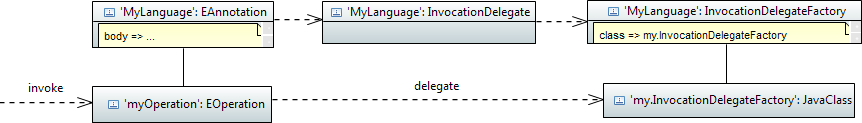
\includegraphics[width=6.75in]{InvocationDelegate.png}
  \end{center}
  \caption{Invocation Delegate example.}
  \label{fig:InvocationDelegate}
\end{figure}

The mechanism is not particularly elegant since it is a protocol for the pre-existing EMF extension capability, without any additional model elements. The body of an Ecore operation can be realized using `MyLanguage':

\begin{verbatim}
<eOperations name="myOperation" ...>
  <eAnnotations source="MyLanguage">
    <details key="body" value="..."/>
  </eAnnotations>
</eOperations>
\end{verbatim}

The `source' of the EAnnotation identifies the purpose of the EAnnotation which contains a mapping from the `body' key to a suitable `value', which is a text string meaningful in `MyLanguage'. The use of `MyLanguage' acquires useful semantics once it is declared to be an invocation delegate for the containing package.

\begin{verbatim}
<eAnnotations source="http://www.eclipse.org/emf/2002/Ecore">
  <details key="invocationDelegates" value="MyLanguage"/>
</eAnnotations>
\end{verbatim}

Defining an  \url{http://www.eclipse.org/emf/2002/Ecore} EAnnotation signals the use of an EMF protocol. The subsequent detail informs EMF that `MyLanguage' is usable as an invocationDelegate.

These declarations contribute to behavior whenever EMF attempts to invoke `myOperation'. This occurs at runtime when an application calls `myOperation' or at generate time when EMF converts a model to Java code. In both cases the invocation of `myOperation' is delegated to the support for `MyLanguage' that may be registered using an Eclipse extension point.

\begin{verbatim}
<extension point="org.eclipse.emf.ecore.invocation_delegate">
  <factory uri="MyLanguage" class="my.InvocationDelegateFactory"/>
</extension>
\end{verbatim}

Provided the `my.InvocationDelegateFactory' Java class correctly supports the relevant EMF APIs, invocation of `myOperation' in the model by any application will delegate to the `MyLanguage' handler without the application being aware that `myOperation' is handled by a `MyLanguage' handler rather than by Java code.

Similar settingDelegate and validationDelegate capabilities support derived property values and class invariants.

\subsection{EMF GenModel Extension}

EMF supports generation of Java code from Ecore models. The generator framework is extensible with the org.eclipse.emf.codegen.ecore.generatorAdapters extension point allowing additional or modified code generation.

\subsection{Eclipse OCL Exploitation and Integration}

The Eclipse UML project uses the Eclipse OCL support as part of its UML to Ecore conversion so that both structural and behavioral aspects of UML models can be realized in Ecore and consequently Java code.

The Eclipse Papyrus (UML diagrams) project exploits Eclipse OCL facilities to validate OCL constraints embedded within UML stereotypes on UML elements to which those stereotypes are applied.

Maintenance of the EMF delegate EAnnotations to embed OCL within Ecore is difficult using an XML editor or the Ecore Tree Editor. Eclipse OCL therefore provides an Xtext-based textual editor that supports definition of model structure and embedded OCL. Figure \ref{fig:OCLinEcore} shows a simple example.
\begin{figure}
  \begin{center}
    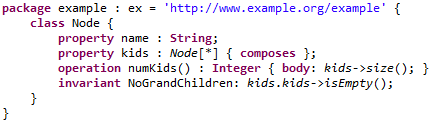
\includegraphics[width=4.0in]{OCLinEcore.png}
  \end{center}
  \caption{OCLinEcore example.}
  \label{fig:OCLinEcore}
\end{figure}

The Eclipse OCL Interactive Console exploits the ability to reuse a selection in another application to support evaluation of OCL queries on objects in other applications.

The Eclipse OCL project supports injecting additional validations defined by Complete OCL documents into other modeling applications.

Eclipse OCL contributes three different `MyLanguage' handlers for the EMF delegates.

\url{http://www.eclipse.org/emf/2002/Ecore/OCL/LPG}: The Classic Eclipse OCL preserves some traditional Eclipse OCL semantics.

\url{http://www.eclipse.org/emf/2002/Ecore/OCL/Pivot}: The Unified or Pivot Eclipse OCL prototypes evolution towards OCL 2.5.

\url{http://www.eclipse.org/emf/2002/Ecore/OCL}: This virtual handler redirects to one of the above according to a user preference.

Eclipse OCL extends the EMF code generation capabilities to support automatic synthesis of Java code for OCL in expressions within Java code.
 
\section{Launching}\label{Launching}

In this section we look at how OCL debugger support can be provided for the OCL integration use cases identified in Section \ref{OCL-Integration} and show how the framework facilities described in Section \ref{Framework-Integration} enable a debugger to be useful.

Launching an OCL debugger to animate the execution of a non-trivial OCL expression requires (at least) two pieces of information
\begin{itemize}
\item The OCL expression to execute
\item The model element to bind to the OCL `self' variable
\item Optionally additional models or parameters
\end{itemize}

(We assume that the model element is supplied by a powerful modeling environment such as EMF so that knowledge of a single model element provides access to all other elements in the same model and to the metamodel of all those elements.) 

This may be compared with a more conventional language, where we may need to know only one piece of information: the program to execute. The program takes responsibility for acquiring further information through an appropriate user interface. Activating a conventional program can therefore be as simple as select and run. Activating a debugger can be nearly as easy; select and debug.

For OCL we may need a double selection to start an independent debugging session. However when problems arise with OCL embedded in another application, we would like to take the OCL debugger to the user's context rather than require the user to reproduce the problem in an independent debugger. Wherever the user's context can be reused, the fidelity of the debugging improves and the additional context needed by the debugger decreases.

In practice there are many ways in which the launch can be achieved with different trade-offs in ease of use and fidelity. These options are summarised in Table \ref{LaunchOptions}.

The model containing instances may be explicitly loaded, may reuse an already loaded version in a changed context, or may use the already loaded version in an unchanged context.

The OCL expression may similarly be loaded, reused or used, but may also be manually entered.

The invocation of the OCL may use the unchanged user's context or a replica of that context.

The execution of the OCL may be supervised by an OCL debugger or a host debugger.

\begin{table}[ht]
\begin{center}
\caption{Launch Options}\label{LaunchOptions}
\bigskip
\begin{tabular}{|l|c|c|c|c|}
\hline
Type & Model & OCL & Invocation & Execution\\ \hline \hline
Independent (\ref{IndependentLaunch}) & load & load & - & OCL debug\\ \hline
Contextual (\ref{ContextualLaunch}) & load & reuse & replica & OCL debug\\ \cline{2-3}
 & reuse & load & & \\ \hline
Console (\ref{ConsoleLaunch}) & reuse & manual & replica & OCL debug\\ \hline
Validity View (\ref{ValidityViewLaunch}) & \multicolumn{2}{|c|}{reuse} & replica & OCL debug\\ \hline
Host (\ref{HostLaunch}) & use & use & use & host/host debug\\ \hline
Automatic (\ref{DelegatedLaunch}) & use & use & use & no/OCL debug\\ \hline
\end{tabular}
\end{center}
\end{table}
 
\subsection{Independent Launch Dialog}\label{IndependentLaunch}

The most general launch approach is a launch dialog that supports the following workflow.

\begin{itemize}
\item Open/Create an OCL Debugger Launch Dialog
\item Select a Model Element within the dialog
\item Select an Expression within the dialog
\item Debug
\end{itemize}

The selections can be facilitated by appropriate browsers that may tailor the available selections to those that exhibit consistent model/metamodel conformance.

The debugger loads the model and the expression and so may fail to reproduce the user scenario accurately.

\subsection{Contextual Launch Dialog}\label{ContextualLaunch}

An abbreviated workflow is available by activating the dialog from an existing model. For instance, selecting a particular Constraint in a UML Diagram and then activating a Debug dialog from the Context menu.

\begin{itemize}
\item Select an Expression within some modeling application
\item Open/Create an OCL Debugger Launch Dialog
\item Select a Model Element within the dialog
\item Debug
\end{itemize}

For this to work, we require the selection in `some modeling application' to be re-usable by the OCL debugger. In Eclipse this is possible because one application can register to listen to selection changes made by any other application.

This contextual launch is more powerful than the independent launch since it re-uses the user's context for one of the two pieces of information. The other piece may need to be reloaded and so may fail to reproduce.

\subsection{Console Launch}\label{ConsoleLaunch}

The ability to discover a user context from a selection underpins the operation of an Interactive OCL Console.

\begin{itemize}
\item Select a Model Element within some modeling application
\item Type an OCL Expression in the Console
\item Execute
\end{itemize}

This workflow is easily changed by replacing `Execute' with `Debug'.

We can successfully re-use the user's model context but must re-type our OCL expressions. If the user's models are evolving or there is any uncertainty as to which model element or expression is causing trouble, this approach still suffers from some loss of the user's problem context.

\subsection{Validity View Launch}\label{ValidityViewLaunch}

A common practical use of OCL involves many model elements that must observe the constraints imposed by many OCL invariants. The formulation of the OCL invariants is assisted by helper operations and derived properties that also involve OCL expressions.

For this use case, the user invokes some form of full or partial Validate action to check that all model elements comply with their constraints. All appropriate constraints are executed on all relevant model elements and the failures are reported to the user. A small number of errors can be reported as a simple list or as decorations on a model diagram or tree. For a larger number of errors and particularly those associated with a defective OCL constraint rather than a defective model, the simple display may not be that helpful. Eclipse OCL therefore provides a Validity View that provides a finer-grained display of both all Constraints per Model Element and all Model Elements per Constraint. Validation results are reported individually for each ModelElement-Constraint combination. In Figure \ref{fig:ValidityView} red/amber/green error/warning/tick icons show the status; the tick boxes are part of the elements-of-interest filtering.

\begin{figure}
  \begin{center}
    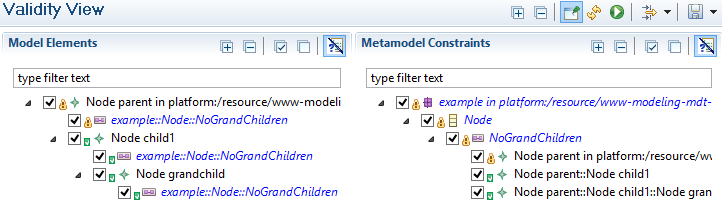
\includegraphics[width=6.75in]{ValidityView.png}
  \end{center}
  \caption{Validity View example.}
  \label{fig:ValidityView}
\end{figure}

This fine-grained display provides no doubt as to where the problem lies and supports the shorter workflow

\begin{itemize}
\item Optionally Run Validation in the Validity View
\item Select a ModelElement-Constraint combination
\item Debug
\end{itemize}

Validation is not normally performed while models are evolving and so this form of launch leaves very limited opportunities to fail to reproduce the user's problem experience. The main hazard is that the activation of the OCL expression does not reuse the original invocation code.

(The Validity View is an extensible facility for which OCL is just an extension. This approach is therefore applicable to other constraint/validation technologies.)

\subsection{Host Debugger Launch}\label{HostLaunch}

Real applications are far too big for users to supervise their invocation and progress. We therefore rely on the use of breakpoints to allow a large application to run and only stop when it reaches an area of interest to the user.

The same is not entirely true of large OCL applications. OCL cannot change anything and so the full requirements of most practical applications cannot be addressed by OCL. We therefore have large non-OCL applications within which there may be many comparatively small OCL contributions. 

Small OCL contributions can be developed and tested in isolation, but the real user problems arise when the full application malfunctions. We therefore need to debug a hybrid application with an outer language, perhaps but not necessarily Java, and inner OCL. Unless we develop a new hybrid debugger, we must use the host debugger for our outer language and we need it to at least collaborate with an OCL debugger for the inner language.

\subsubsection{OCL interpreted and debugged in the host language}

A very simple solution is available when the OCL tooling uses the same language as the outer language. The user can just step through the inner code using the outer language. Unfortunately this may require many hundreds of outer language steps to progress a single equivalent OCL step. The displayed source code is hard to understand. This approach is therefore a last resort suitable only for the developers of the OCL tooling.

\subsubsection{OCL interpreted and debugged via the host language}

Debugger frameworks allow for a variety of source renderings such as assembler level, source level, pre-process level. It should therefore be possible to enhance a host debugger to behave usefully at an OCL source level.

This approach has not yet been pursued by Eclipse OCL whose debugger extends the basic Eclipse Debugger Framework. The Eclipse Java Debugger provides many enhancements to this framework. It may be relatively simple to promote the Eclipse OCL debugger to the enhanced framework once the enhancements are fully understood. 

\subsubsection{OCL compiled in the host language}

Eclipse OCL provides an OCL to Java code generator and so the inner OCL may be expressed in Java to significantly improve performance. Debugging the auto-generated code may then involve less than ten outer language steps per equivalent OCL step. This is a significant improvement over hundreds but auto-generated optimized source code is not always readable.

Enhancing the Eclipse Java debugger to provide an OCL view of the auto-generated code has not yet been attempted.

\subsection{Automatic Delegated Launch}\label{DelegatedLaunch}

The three preceding host approaches all involve launching an outer language host debugger and attempting to use it to debug inner OCL. Quite apart from the need to enhance the outer language debugger, a debugger has to be launched in order to have it available when the user problem is encountered. For major Eclipse applications this may require that the entire Eclipse application is run under the control of a debugger in another Eclipse session. It is not possible to run the outer application normally and start an OCL debugger automatically for an OCL problem.

EMF-delegates provide an alternative solution. The program control flow from the outer application to the inner OCL is orchestrated by the EMF delegates and so an alternative delegation implementation may activate an OCL debugger. The outer code may be run normally and since it is unaware of the underlying delegate implementation approach, the outer code is unaffected by the `activation' of the debugger. The debugger for the inner OCL starts supervision as soon as the inner OCL is invoked. Execution may stop immediately or at a breakpoint. In practice enabling/disabling debug in outer applications can be achieved by adjusting the user preference to redirect the virtual OCL delegate to the debug delegate.

\url{http://www.eclipse.org/emf/2002/Ecore/OCL/Debug}

\section{Related Work}\label{Related-Work}

The EMF delegates functionality is over four years old but write ups have been limited to Wiki pages\cite{OCLinEcore} and Eclipse OCL documentation.

Dresden OCL\cite{DresdenOCL-Debug} introduced the first OCL debugger exploiting the Eclipse Debugger Framework. Although Dresden OCL uses EMF, it does not exploit the integration opportunities outlined in Section \ref{Framework-Integration}. Dresden OCL tooling is therefore limited to the independent use case. Larger applications such as MagicDraw may make use of the APIs.

The Eclipse OCL debugger also exploits the Eclipse Debugger Framework and so has many similarities to the Dresden OCL debugger including deferring more challenging facilities such as Watchpoints to a future release. Eclipse OCL does exploit the EMF integration opportunities and so the Eclipse OCL debugger may be used in embedded applications. The Luna release \cite{OCL-Luna} supports the Independent, Integrated, Extended and Compiled use cases outlined in Table \ref{IntegrationOptions} and the Independent, Contextual, Console and Validity View use cases outlined in Table \ref{LaunchOptions}. Support for the Automatic use case was developed while writing this paper.

A third widely used OCL tool, USE \cite{USE}, does not use EMF; USE provides its own framework with which it provides interesting tools including an OCL stepper; a precursor to an OCL debugger.

The need for a debugger was highlighted by IDE4OCL\cite{Chimiak-Opaka}, but perhaps because it was so obvious that a debugger was required, little attention was paid to how a debugger might actually be used.

\section{Conclusions}\label{Conclusion}
We have identified a variety of ways in which OCL may be used in practice, and noted that those that support integration with applications require the application to either exploit OCL toolkit APIs explicitly or to use a more generally extensible framework that may support implicit use of OCL.

We have identified characteristics of EMF that support extension by OCL toolkits.

We have identified how an OCL debugger can be launched for different OCL use cases.

We have explained how Eclipse OCL exploits the extensibility of EMF to support embedding OCL within larger applications and how the Eclipse OCL debugger may be used to debug these larger embedded applications.

\paragraph{Acknowledgements}

Many thanks to Adolfo Sanchez-Barbudo Herrera for helpful comments.

%\bibliographystyle{alpha} 
%\bibliography{samplebib}
%inline the .bbl file directly for mailing to authors.

\begin{thebibliography}{11}

\bibitem{OCL-2.4} Object Constraint Language. Version 2.4., OMG Document Number: formal/2014-02-03, Object Management Group (2009),  \url{http://www.omg.org/spec/OCL/2.4}

\bibitem{DresdenOCL-Debug} Sch\"utze, L., Wilke, C., Demuth, B.: Tool-Supported Step-By-Step Debugging
for the Object Constraint Language, OCL 2013, International Workshop on OCL and Textual Modelling, MODELS 2013, Miami

\bibitem{Chimiak-Opaka} Chimiak-Opaka, J., Demuth, B.: A Feature Model for an IDE4OCL, OCL 2010: Workshop on OCL and Textual Modelling, Models 2010, Oslo"

\bibitem{UML-2.5} OMG Unified Modeling Language (OMG UML), Version 2.5 Beta2, {OMG Document Number}: ptc/2013-09-05, Object Management Group (2013), \url{http://www.omg.org/spec/UML/2.5/Beta2}

\bibitem{EMF} The Eclipse Modeling Framework Project \url{http://www.eclipse.org/emf}

\bibitem{QVT-1.2} Query/View/Transformation Specification, Version 1.2 Beta, {OMG Document Number}: ptc/2014-03-38, 2014, Object Management Group (2014) \url{http://www.omg.org/spec/QVT/1.2/}

\bibitem{MOFM2T} MOF Model to Text Transformation Language,  v1.0, {OMG Document Number}: formal/2008-01-16, Object Management Group (2008), \url{http://www.omg.org/spec/MOFM2T/1.0"}

\bibitem{OCL-Luna} Eclipse OCL 5.0.1, Luna release, June 2014, \url{http://www.eclipse.org/modeling/download.php?file=/modeling/mdt/ocl/downloads/drops/5.0.1/R201406230143/mdt-ocl-Update-5.0.1.zip}

\bibitem{OCLinEcore} OCLinEcore Wiki page, 2010, \url{http://wiki.eclipse.org/index.php?title=OCL/OCLinEcore}

\bibitem{USE} UML-based Specification Environment, \url{http://sourceforge.net/projects/useocl/}

\end{thebibliography}

\end{document}


